\begin{figure}[H] \centering % Created by tikzDevice version 0.12.4 on 2023-07-23 21:21:37
% !TEX encoding = UTF-8 Unicode
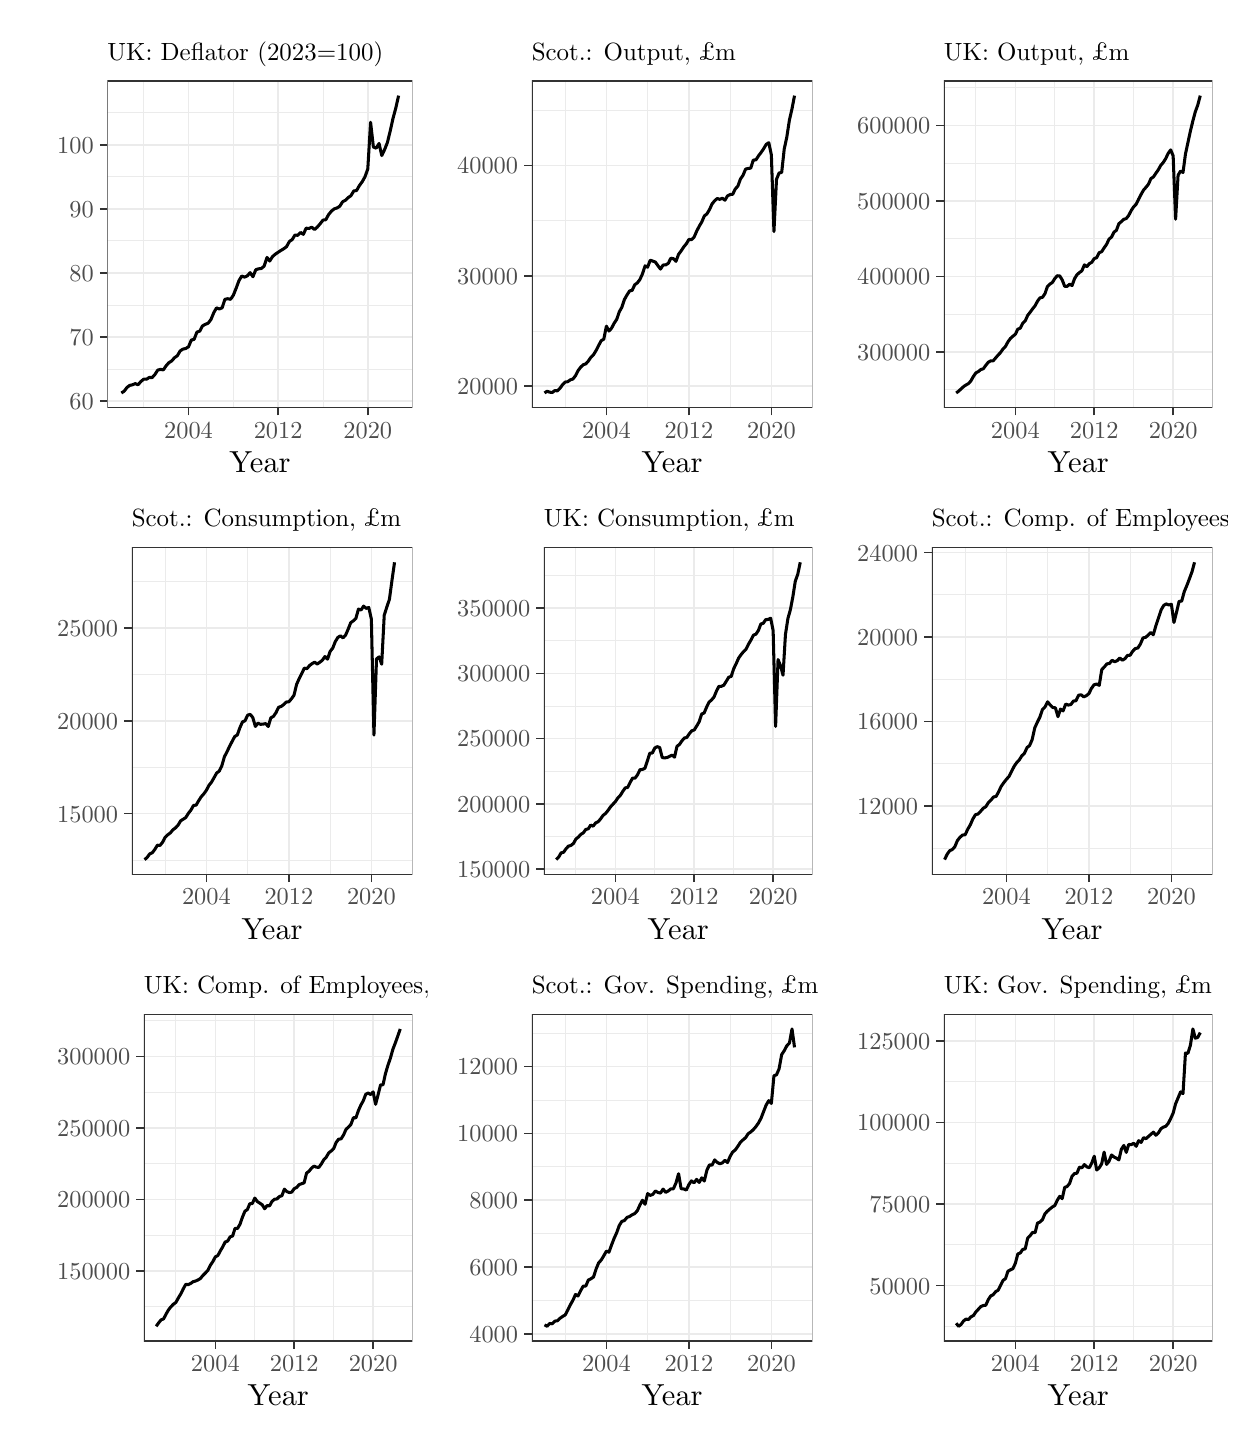
\begin{tikzpicture}[x=1pt,y=1pt]
\definecolor{fillColor}{RGB}{255,255,255}
\path[use as bounding box,fill=fillColor,fill opacity=0.00] (0,0) rectangle (433.62,505.89);
\begin{scope}
\path[clip] (  0.00,337.26) rectangle (144.54,505.89);
\definecolor{drawColor}{RGB}{255,255,255}
\definecolor{fillColor}{RGB}{255,255,255}

\path[draw=drawColor,line width= 0.6pt,line join=round,line cap=round,fill=fillColor] (  0.00,337.26) rectangle (144.54,505.89);
\end{scope}
\begin{scope}
\path[clip] ( 28.83,368.51) rectangle (139.04,486.70);
\definecolor{fillColor}{RGB}{255,255,255}

\path[fill=fillColor] ( 28.83,368.51) rectangle (139.04,486.70);
\definecolor{drawColor}{gray}{0.92}

\path[draw=drawColor,line width= 0.3pt,line join=round] ( 28.83,382.53) --
	(139.04,382.53);

\path[draw=drawColor,line width= 0.3pt,line join=round] ( 28.83,405.69) --
	(139.04,405.69);

\path[draw=drawColor,line width= 0.3pt,line join=round] ( 28.83,428.85) --
	(139.04,428.85);

\path[draw=drawColor,line width= 0.3pt,line join=round] ( 28.83,452.02) --
	(139.04,452.02);

\path[draw=drawColor,line width= 0.3pt,line join=round] ( 28.83,475.18) --
	(139.04,475.18);

\path[draw=drawColor,line width= 0.3pt,line join=round] ( 41.93,368.51) --
	( 41.93,486.70);

\path[draw=drawColor,line width= 0.3pt,line join=round] ( 74.32,368.51) --
	( 74.32,486.70);

\path[draw=drawColor,line width= 0.3pt,line join=round] (106.71,368.51) --
	(106.71,486.70);

\path[draw=drawColor,line width= 0.6pt,line join=round] ( 28.83,370.95) --
	(139.04,370.95);

\path[draw=drawColor,line width= 0.6pt,line join=round] ( 28.83,394.11) --
	(139.04,394.11);

\path[draw=drawColor,line width= 0.6pt,line join=round] ( 28.83,417.27) --
	(139.04,417.27);

\path[draw=drawColor,line width= 0.6pt,line join=round] ( 28.83,440.43) --
	(139.04,440.43);

\path[draw=drawColor,line width= 0.6pt,line join=round] ( 28.83,463.60) --
	(139.04,463.60);

\path[draw=drawColor,line width= 0.6pt,line join=round] ( 58.12,368.51) --
	( 58.12,486.70);

\path[draw=drawColor,line width= 0.6pt,line join=round] ( 90.51,368.51) --
	( 90.51,486.70);

\path[draw=drawColor,line width= 0.6pt,line join=round] (122.90,368.51) --
	(122.90,486.70);
\definecolor{drawColor}{RGB}{0,0,0}

\path[draw=drawColor,line width= 1.1pt,line join=round] ( 33.84,373.89) --
	( 34.83,374.49) --
	( 35.84,375.83) --
	( 36.86,376.62) --
	( 37.88,376.84) --
	( 38.88,377.26) --
	( 39.89,376.86) --
	( 40.91,378.04) --
	( 41.93,378.86) --
	( 42.94,378.85) --
	( 43.94,379.50) --
	( 44.96,379.44) --
	( 45.98,380.56) --
	( 46.98,382.13) --
	( 47.99,382.42) --
	( 49.01,382.22) --
	( 50.03,383.71) --
	( 51.03,384.84) --
	( 52.04,385.45) --
	( 53.06,386.63) --
	( 54.08,387.34) --
	( 55.07,389.04) --
	( 56.08,389.73) --
	( 57.10,389.95) --
	( 58.12,390.57) --
	( 59.13,393.01) --
	( 60.14,393.26) --
	( 61.16,395.90) --
	( 62.18,396.23) --
	( 63.18,398.14) --
	( 64.19,398.69) --
	( 65.21,399.08) --
	( 66.23,400.43) --
	( 67.22,402.84) --
	( 68.23,404.63) --
	( 69.25,404.24) --
	( 70.27,404.65) --
	( 71.27,407.74) --
	( 72.28,407.94) --
	( 73.30,407.73) --
	( 74.32,409.22) --
	( 75.33,411.74) --
	( 76.33,414.43) --
	( 77.35,416.15) --
	( 78.37,415.75) --
	( 79.37,416.20) --
	( 80.38,417.36) --
	( 81.40,415.88) --
	( 82.42,418.41) --
	( 83.42,418.74) --
	( 84.43,418.87) --
	( 85.45,419.72) --
	( 86.47,422.86) --
	( 87.46,421.57) --
	( 88.47,423.16) --
	( 89.49,424.05) --
	( 90.51,424.74) --
	( 91.52,425.40) --
	( 92.53,426.00) --
	( 93.55,426.77) --
	( 94.57,428.62) --
	( 95.57,429.31) --
	( 96.58,430.94) --
	( 97.59,430.85) --
	( 98.61,431.89) --
	( 99.61,431.20) --
	(100.62,433.44) --
	(101.64,433.32) --
	(102.66,433.78) --
	(103.66,432.92) --
	(104.67,433.84) --
	(105.69,435.03) --
	(106.71,436.35) --
	(107.72,436.49) --
	(108.72,438.31) --
	(109.74,439.57) --
	(110.76,440.40) --
	(111.76,440.74) --
	(112.77,441.35) --
	(113.79,442.98) --
	(114.81,443.50) --
	(115.81,444.47) --
	(116.82,445.18) --
	(117.84,446.88) --
	(118.86,447.05) --
	(119.85,448.82) --
	(120.86,450.18) --
	(121.88,451.99) --
	(122.90,454.85) --
	(123.91,471.71) --
	(124.92,462.76) --
	(125.94,462.34) --
	(126.96,464.03) --
	(127.96,459.67) --
	(128.96,461.80) --
	(129.98,464.38) --
	(131.00,468.53) --
	(132.00,473.07) --
	(133.01,476.79) --
	(134.03,481.33);
\definecolor{drawColor}{gray}{0.20}

\path[draw=drawColor,line width= 0.6pt,line join=round,line cap=round] ( 28.83,368.51) rectangle (139.04,486.70);
\end{scope}
\begin{scope}
\path[clip] (  0.00,  0.00) rectangle (433.62,505.89);
\definecolor{drawColor}{gray}{0.30}

\node[text=drawColor,anchor=base east,inner sep=0pt, outer sep=0pt, scale=  0.88] at ( 23.88,367.92) { 60};

\node[text=drawColor,anchor=base east,inner sep=0pt, outer sep=0pt, scale=  0.88] at ( 23.88,391.08) { 70};

\node[text=drawColor,anchor=base east,inner sep=0pt, outer sep=0pt, scale=  0.88] at ( 23.88,414.24) { 80};

\node[text=drawColor,anchor=base east,inner sep=0pt, outer sep=0pt, scale=  0.88] at ( 23.88,437.40) { 90};

\node[text=drawColor,anchor=base east,inner sep=0pt, outer sep=0pt, scale=  0.88] at ( 23.88,460.57) {100};
\end{scope}
\begin{scope}
\path[clip] (  0.00,  0.00) rectangle (433.62,505.89);
\definecolor{drawColor}{gray}{0.20}

\path[draw=drawColor,line width= 0.6pt,line join=round] ( 26.08,370.95) --
	( 28.83,370.95);

\path[draw=drawColor,line width= 0.6pt,line join=round] ( 26.08,394.11) --
	( 28.83,394.11);

\path[draw=drawColor,line width= 0.6pt,line join=round] ( 26.08,417.27) --
	( 28.83,417.27);

\path[draw=drawColor,line width= 0.6pt,line join=round] ( 26.08,440.43) --
	( 28.83,440.43);

\path[draw=drawColor,line width= 0.6pt,line join=round] ( 26.08,463.60) --
	( 28.83,463.60);
\end{scope}
\begin{scope}
\path[clip] (  0.00,  0.00) rectangle (433.62,505.89);
\definecolor{drawColor}{gray}{0.20}

\path[draw=drawColor,line width= 0.6pt,line join=round] ( 58.12,365.76) --
	( 58.12,368.51);

\path[draw=drawColor,line width= 0.6pt,line join=round] ( 90.51,365.76) --
	( 90.51,368.51);

\path[draw=drawColor,line width= 0.6pt,line join=round] (122.90,365.76) --
	(122.90,368.51);
\end{scope}
\begin{scope}
\path[clip] (  0.00,  0.00) rectangle (433.62,505.89);
\definecolor{drawColor}{gray}{0.30}

\node[text=drawColor,anchor=base,inner sep=0pt, outer sep=0pt, scale=  0.88] at ( 58.12,357.50) {2004};

\node[text=drawColor,anchor=base,inner sep=0pt, outer sep=0pt, scale=  0.88] at ( 90.51,357.50) {2012};

\node[text=drawColor,anchor=base,inner sep=0pt, outer sep=0pt, scale=  0.88] at (122.90,357.50) {2020};
\end{scope}
\begin{scope}
\path[clip] (  0.00,  0.00) rectangle (433.62,505.89);
\definecolor{drawColor}{RGB}{0,0,0}

\node[text=drawColor,anchor=base,inner sep=0pt, outer sep=0pt, scale=  1.10] at ( 83.93,345.19) {Year};
\end{scope}
\begin{scope}
\path[clip] (  0.00,  0.00) rectangle (433.62,505.89);
\definecolor{drawColor}{RGB}{0,0,0}

\node[text=drawColor,anchor=base west,inner sep=0pt, outer sep=0pt, scale=  0.90] at ( 28.83,494.19) {UK: Deflator (2023=100)};
\end{scope}
\begin{scope}
\path[clip] (144.54,337.26) rectangle (289.08,505.89);
\definecolor{drawColor}{RGB}{255,255,255}
\definecolor{fillColor}{RGB}{255,255,255}

\path[draw=drawColor,line width= 0.6pt,line join=round,line cap=round,fill=fillColor] (144.54,337.26) rectangle (289.08,505.89);
\end{scope}
\begin{scope}
\path[clip] (182.16,368.51) rectangle (283.58,486.70);
\definecolor{fillColor}{RGB}{255,255,255}

\path[fill=fillColor] (182.16,368.51) rectangle (283.58,486.70);
\definecolor{drawColor}{gray}{0.92}

\path[draw=drawColor,line width= 0.3pt,line join=round] (182.16,396.24) --
	(283.58,396.24);

\path[draw=drawColor,line width= 0.3pt,line join=round] (182.16,436.13) --
	(283.58,436.13);

\path[draw=drawColor,line width= 0.3pt,line join=round] (182.16,476.01) --
	(283.58,476.01);

\path[draw=drawColor,line width= 0.3pt,line join=round] (194.22,368.51) --
	(194.22,486.70);

\path[draw=drawColor,line width= 0.3pt,line join=round] (224.02,368.51) --
	(224.02,486.70);

\path[draw=drawColor,line width= 0.3pt,line join=round] (253.83,368.51) --
	(253.83,486.70);

\path[draw=drawColor,line width= 0.6pt,line join=round] (182.16,376.30) --
	(283.58,376.30);

\path[draw=drawColor,line width= 0.6pt,line join=round] (182.16,416.19) --
	(283.58,416.19);

\path[draw=drawColor,line width= 0.6pt,line join=round] (182.16,456.07) --
	(283.58,456.07);

\path[draw=drawColor,line width= 0.6pt,line join=round] (209.12,368.51) --
	(209.12,486.70);

\path[draw=drawColor,line width= 0.6pt,line join=round] (238.93,368.51) --
	(238.93,486.70);

\path[draw=drawColor,line width= 0.6pt,line join=round] (268.73,368.51) --
	(268.73,486.70);
\definecolor{drawColor}{RGB}{0,0,0}

\path[draw=drawColor,line width= 1.1pt,line join=round] (186.77,373.89) --
	(187.69,374.50) --
	(188.62,374.18) --
	(189.56,374.05) --
	(190.50,374.76) --
	(191.41,374.64) --
	(192.34,375.55) --
	(193.28,376.89) --
	(194.22,377.83) --
	(195.15,377.96) --
	(196.08,378.63) --
	(197.01,378.92) --
	(197.95,380.11) --
	(198.87,381.93) --
	(199.80,383.18) --
	(200.74,384.08) --
	(201.68,384.40) --
	(202.59,385.42) --
	(203.52,386.78) --
	(204.46,387.71) --
	(205.40,389.25) --
	(206.32,391.06) --
	(207.24,392.77) --
	(208.18,393.32) --
	(209.12,398.01) --
	(210.05,396.27) --
	(210.98,397.28) --
	(211.92,399.11) --
	(212.85,400.48) --
	(213.77,403.21) --
	(214.70,404.85) --
	(215.64,407.67) --
	(216.58,409.32) --
	(217.50,410.75) --
	(218.42,410.95) --
	(219.36,412.98) --
	(220.30,413.66) --
	(221.22,414.87) --
	(222.15,416.92) --
	(223.09,419.81) --
	(224.02,419.35) --
	(224.95,421.86) --
	(225.88,421.54) --
	(226.82,421.19) --
	(227.76,419.85) --
	(228.67,418.65) --
	(229.60,420.11) --
	(230.54,420.17) --
	(231.48,420.72) --
	(232.40,422.58) --
	(233.33,422.41) --
	(234.26,421.45) --
	(235.20,424.00) --
	(236.12,425.21) --
	(237.05,426.64) --
	(237.99,427.76) --
	(238.93,429.37) --
	(239.85,429.29) --
	(240.78,430.13) --
	(241.72,432.30) --
	(242.66,434.13) --
	(243.58,435.67) --
	(244.50,437.84) --
	(245.44,438.60) --
	(246.38,440.15) --
	(247.30,442.20) --
	(248.23,443.34) --
	(249.17,444.16) --
	(250.10,443.85) --
	(251.02,444.25) --
	(251.95,443.54) --
	(252.89,445.11) --
	(253.83,445.59) --
	(254.76,445.67) --
	(255.68,447.60) --
	(256.62,448.61) --
	(257.56,451.21) --
	(258.48,452.51) --
	(259.41,454.77) --
	(260.35,455.03) --
	(261.28,455.12) --
	(262.20,458.05) --
	(263.13,458.09) --
	(264.07,459.55) --
	(265.01,460.78) --
	(265.92,462.12) --
	(266.85,463.69) --
	(267.79,464.33) --
	(268.73,459.92) --
	(269.66,432.20) --
	(270.59,451.10) --
	(271.52,453.37) --
	(272.46,453.58) --
	(273.38,462.03) --
	(274.31,466.35) --
	(275.25,472.47) --
	(276.19,476.59) --
	(277.10,481.33);
\definecolor{drawColor}{gray}{0.20}

\path[draw=drawColor,line width= 0.6pt,line join=round,line cap=round] (182.16,368.51) rectangle (283.58,486.70);
\end{scope}
\begin{scope}
\path[clip] (  0.00,  0.00) rectangle (433.62,505.89);
\definecolor{drawColor}{gray}{0.30}

\node[text=drawColor,anchor=base east,inner sep=0pt, outer sep=0pt, scale=  0.88] at (177.21,373.27) {20000};

\node[text=drawColor,anchor=base east,inner sep=0pt, outer sep=0pt, scale=  0.88] at (177.21,413.15) {30000};

\node[text=drawColor,anchor=base east,inner sep=0pt, outer sep=0pt, scale=  0.88] at (177.21,453.04) {40000};
\end{scope}
\begin{scope}
\path[clip] (  0.00,  0.00) rectangle (433.62,505.89);
\definecolor{drawColor}{gray}{0.20}

\path[draw=drawColor,line width= 0.6pt,line join=round] (179.41,376.30) --
	(182.16,376.30);

\path[draw=drawColor,line width= 0.6pt,line join=round] (179.41,416.19) --
	(182.16,416.19);

\path[draw=drawColor,line width= 0.6pt,line join=round] (179.41,456.07) --
	(182.16,456.07);
\end{scope}
\begin{scope}
\path[clip] (  0.00,  0.00) rectangle (433.62,505.89);
\definecolor{drawColor}{gray}{0.20}

\path[draw=drawColor,line width= 0.6pt,line join=round] (209.12,365.76) --
	(209.12,368.51);

\path[draw=drawColor,line width= 0.6pt,line join=round] (238.93,365.76) --
	(238.93,368.51);

\path[draw=drawColor,line width= 0.6pt,line join=round] (268.73,365.76) --
	(268.73,368.51);
\end{scope}
\begin{scope}
\path[clip] (  0.00,  0.00) rectangle (433.62,505.89);
\definecolor{drawColor}{gray}{0.30}

\node[text=drawColor,anchor=base,inner sep=0pt, outer sep=0pt, scale=  0.88] at (209.12,357.50) {2004};

\node[text=drawColor,anchor=base,inner sep=0pt, outer sep=0pt, scale=  0.88] at (238.93,357.50) {2012};

\node[text=drawColor,anchor=base,inner sep=0pt, outer sep=0pt, scale=  0.88] at (268.73,357.50) {2020};
\end{scope}
\begin{scope}
\path[clip] (  0.00,  0.00) rectangle (433.62,505.89);
\definecolor{drawColor}{RGB}{0,0,0}

\node[text=drawColor,anchor=base,inner sep=0pt, outer sep=0pt, scale=  1.10] at (232.87,345.19) {Year};
\end{scope}
\begin{scope}
\path[clip] (  0.00,  0.00) rectangle (433.62,505.89);
\definecolor{drawColor}{RGB}{0,0,0}

\node[text=drawColor,anchor=base west,inner sep=0pt, outer sep=0pt, scale=  0.90] at (182.16,494.19) {Scot.: Output, £m};
\end{scope}
\begin{scope}
\path[clip] (289.08,337.26) rectangle (433.62,505.89);
\definecolor{drawColor}{RGB}{255,255,255}
\definecolor{fillColor}{RGB}{255,255,255}

\path[draw=drawColor,line width= 0.6pt,line join=round,line cap=round,fill=fillColor] (289.08,337.26) rectangle (433.62,505.89);
\end{scope}
\begin{scope}
\path[clip] (331.10,368.51) rectangle (428.12,486.70);
\definecolor{fillColor}{RGB}{255,255,255}

\path[fill=fillColor] (331.10,368.51) rectangle (428.12,486.70);
\definecolor{drawColor}{gray}{0.92}

\path[draw=drawColor,line width= 0.3pt,line join=round] (331.10,375.04) --
	(428.12,375.04);

\path[draw=drawColor,line width= 0.3pt,line join=round] (331.10,402.32) --
	(428.12,402.32);

\path[draw=drawColor,line width= 0.3pt,line join=round] (331.10,429.60) --
	(428.12,429.60);

\path[draw=drawColor,line width= 0.3pt,line join=round] (331.10,456.88) --
	(428.12,456.88);

\path[draw=drawColor,line width= 0.3pt,line join=round] (331.10,484.16) --
	(428.12,484.16);

\path[draw=drawColor,line width= 0.3pt,line join=round] (342.64,368.51) --
	(342.64,486.70);

\path[draw=drawColor,line width= 0.3pt,line join=round] (371.15,368.51) --
	(371.15,486.70);

\path[draw=drawColor,line width= 0.3pt,line join=round] (399.66,368.51) --
	(399.66,486.70);

\path[draw=drawColor,line width= 0.6pt,line join=round] (331.10,388.68) --
	(428.12,388.68);

\path[draw=drawColor,line width= 0.6pt,line join=round] (331.10,415.96) --
	(428.12,415.96);

\path[draw=drawColor,line width= 0.6pt,line join=round] (331.10,443.24) --
	(428.12,443.24);

\path[draw=drawColor,line width= 0.6pt,line join=round] (331.10,470.52) --
	(428.12,470.52);

\path[draw=drawColor,line width= 0.6pt,line join=round] (356.89,368.51) --
	(356.89,486.70);

\path[draw=drawColor,line width= 0.6pt,line join=round] (385.40,368.51) --
	(385.40,486.70);

\path[draw=drawColor,line width= 0.6pt,line join=round] (413.91,368.51) --
	(413.91,486.70);
\definecolor{drawColor}{RGB}{0,0,0}

\path[draw=drawColor,line width= 1.1pt,line join=round] (335.51,373.89) --
	(336.39,374.53) --
	(337.28,375.37) --
	(338.18,376.18) --
	(339.07,376.78) --
	(339.95,377.27) --
	(340.84,378.26) --
	(341.74,379.88) --
	(342.64,381.14) --
	(343.52,381.63) --
	(344.41,382.34) --
	(345.31,382.63) --
	(346.21,383.86) --
	(347.08,384.96) --
	(347.97,385.48) --
	(348.87,385.49) --
	(349.77,386.55) --
	(350.65,387.57) --
	(351.53,388.48) --
	(352.43,389.80) --
	(353.33,390.71) --
	(354.21,392.35) --
	(355.10,393.57) --
	(355.99,394.37) --
	(356.89,395.10) --
	(357.78,396.94) --
	(358.67,397.29) --
	(359.56,399.06) --
	(360.46,399.94) --
	(361.34,401.91) --
	(362.23,403.05) --
	(363.13,404.28) --
	(364.02,405.40) --
	(364.90,407.05) --
	(365.79,408.24) --
	(366.69,408.45) --
	(367.59,409.76) --
	(368.46,412.29) --
	(369.35,413.22) --
	(370.25,413.79) --
	(371.15,415.22) --
	(372.03,416.24) --
	(372.92,416.19) --
	(373.82,414.76) --
	(374.72,412.43) --
	(375.60,412.39) --
	(376.48,413.19) --
	(377.38,412.70) --
	(378.28,415.18) --
	(379.16,416.61) --
	(380.05,417.39) --
	(380.94,418.04) --
	(381.84,420.18) --
	(382.72,419.49) --
	(383.61,420.60) --
	(384.50,421.09) --
	(385.40,422.44) --
	(386.29,422.78) --
	(387.18,424.58) --
	(388.08,424.93) --
	(388.97,426.33) --
	(389.85,427.56) --
	(390.74,429.48) --
	(391.64,430.20) --
	(392.54,432.01) --
	(393.41,432.67) --
	(394.30,435.05) --
	(395.20,435.81) --
	(396.10,436.64) --
	(396.97,436.91) --
	(397.86,438.06) --
	(398.76,439.81) --
	(399.66,441.17) --
	(400.55,442.10) --
	(401.43,443.91) --
	(402.33,445.64) --
	(403.23,447.23) --
	(404.11,448.21) --
	(405.00,449.35) --
	(405.89,451.37) --
	(406.79,451.94) --
	(407.67,453.27) --
	(408.56,454.57) --
	(409.45,456.14) --
	(410.35,457.19) --
	(411.23,458.60) --
	(412.12,460.48) --
	(413.02,461.72) --
	(413.91,459.59) --
	(414.80,436.65) --
	(415.69,452.56) --
	(416.59,454.06) --
	(417.48,453.58) --
	(418.36,460.22) --
	(419.25,464.35) --
	(420.15,468.54) --
	(421.05,472.23) --
	(421.92,475.49) --
	(422.81,477.93) --
	(423.71,481.33);
\definecolor{drawColor}{gray}{0.20}

\path[draw=drawColor,line width= 0.6pt,line join=round,line cap=round] (331.10,368.51) rectangle (428.12,486.70);
\end{scope}
\begin{scope}
\path[clip] (  0.00,  0.00) rectangle (433.62,505.89);
\definecolor{drawColor}{gray}{0.30}

\node[text=drawColor,anchor=base east,inner sep=0pt, outer sep=0pt, scale=  0.88] at (326.15,385.65) {300000};

\node[text=drawColor,anchor=base east,inner sep=0pt, outer sep=0pt, scale=  0.88] at (326.15,412.93) {400000};

\node[text=drawColor,anchor=base east,inner sep=0pt, outer sep=0pt, scale=  0.88] at (326.15,440.21) {500000};

\node[text=drawColor,anchor=base east,inner sep=0pt, outer sep=0pt, scale=  0.88] at (326.15,467.49) {600000};
\end{scope}
\begin{scope}
\path[clip] (  0.00,  0.00) rectangle (433.62,505.89);
\definecolor{drawColor}{gray}{0.20}

\path[draw=drawColor,line width= 0.6pt,line join=round] (328.35,388.68) --
	(331.10,388.68);

\path[draw=drawColor,line width= 0.6pt,line join=round] (328.35,415.96) --
	(331.10,415.96);

\path[draw=drawColor,line width= 0.6pt,line join=round] (328.35,443.24) --
	(331.10,443.24);

\path[draw=drawColor,line width= 0.6pt,line join=round] (328.35,470.52) --
	(331.10,470.52);
\end{scope}
\begin{scope}
\path[clip] (  0.00,  0.00) rectangle (433.62,505.89);
\definecolor{drawColor}{gray}{0.20}

\path[draw=drawColor,line width= 0.6pt,line join=round] (356.89,365.76) --
	(356.89,368.51);

\path[draw=drawColor,line width= 0.6pt,line join=round] (385.40,365.76) --
	(385.40,368.51);

\path[draw=drawColor,line width= 0.6pt,line join=round] (413.91,365.76) --
	(413.91,368.51);
\end{scope}
\begin{scope}
\path[clip] (  0.00,  0.00) rectangle (433.62,505.89);
\definecolor{drawColor}{gray}{0.30}

\node[text=drawColor,anchor=base,inner sep=0pt, outer sep=0pt, scale=  0.88] at (356.89,357.50) {2004};

\node[text=drawColor,anchor=base,inner sep=0pt, outer sep=0pt, scale=  0.88] at (385.40,357.50) {2012};

\node[text=drawColor,anchor=base,inner sep=0pt, outer sep=0pt, scale=  0.88] at (413.91,357.50) {2020};
\end{scope}
\begin{scope}
\path[clip] (  0.00,  0.00) rectangle (433.62,505.89);
\definecolor{drawColor}{RGB}{0,0,0}

\node[text=drawColor,anchor=base,inner sep=0pt, outer sep=0pt, scale=  1.10] at (379.61,345.19) {Year};
\end{scope}
\begin{scope}
\path[clip] (  0.00,  0.00) rectangle (433.62,505.89);
\definecolor{drawColor}{RGB}{0,0,0}

\node[text=drawColor,anchor=base west,inner sep=0pt, outer sep=0pt, scale=  0.90] at (331.10,494.19) {UK: Output, £m};
\end{scope}
\begin{scope}
\path[clip] (  0.00,168.63) rectangle (144.54,337.26);
\definecolor{drawColor}{RGB}{255,255,255}
\definecolor{fillColor}{RGB}{255,255,255}

\path[draw=drawColor,line width= 0.6pt,line join=round,line cap=round,fill=fillColor] (  0.00,168.63) rectangle (144.54,337.26);
\end{scope}
\begin{scope}
\path[clip] ( 37.62,199.88) rectangle (139.04,318.07);
\definecolor{fillColor}{RGB}{255,255,255}

\path[fill=fillColor] ( 37.62,199.88) rectangle (139.04,318.07);
\definecolor{drawColor}{gray}{0.92}

\path[draw=drawColor,line width= 0.3pt,line join=round] ( 37.62,205.12) --
	(139.04,205.12);

\path[draw=drawColor,line width= 0.3pt,line join=round] ( 37.62,238.64) --
	(139.04,238.64);

\path[draw=drawColor,line width= 0.3pt,line join=round] ( 37.62,272.15) --
	(139.04,272.15);

\path[draw=drawColor,line width= 0.3pt,line join=round] ( 37.62,305.67) --
	(139.04,305.67);

\path[draw=drawColor,line width= 0.3pt,line join=round] ( 49.68,199.88) --
	( 49.68,318.07);

\path[draw=drawColor,line width= 0.3pt,line join=round] ( 79.48,199.88) --
	( 79.48,318.07);

\path[draw=drawColor,line width= 0.3pt,line join=round] (109.29,199.88) --
	(109.29,318.07);

\path[draw=drawColor,line width= 0.6pt,line join=round] ( 37.62,221.88) --
	(139.04,221.88);

\path[draw=drawColor,line width= 0.6pt,line join=round] ( 37.62,255.40) --
	(139.04,255.40);

\path[draw=drawColor,line width= 0.6pt,line join=round] ( 37.62,288.91) --
	(139.04,288.91);

\path[draw=drawColor,line width= 0.6pt,line join=round] ( 64.58,199.88) --
	( 64.58,318.07);

\path[draw=drawColor,line width= 0.6pt,line join=round] ( 94.39,199.88) --
	( 94.39,318.07);

\path[draw=drawColor,line width= 0.6pt,line join=round] (124.19,199.88) --
	(124.19,318.07);
\definecolor{drawColor}{RGB}{0,0,0}

\path[draw=drawColor,line width= 1.1pt,line join=round] ( 42.23,205.26) --
	( 43.15,206.03) --
	( 44.08,207.32) --
	( 45.02,207.75) --
	( 45.96,208.97) --
	( 46.87,210.47) --
	( 47.80,210.37) --
	( 48.74,211.54) --
	( 49.68,213.35) --
	( 50.61,214.23) --
	( 51.54,214.91) --
	( 52.47,216.02) --
	( 53.41,216.72) --
	( 54.33,217.70) --
	( 55.26,219.25) --
	( 56.20,219.87) --
	( 57.14,220.48) --
	( 58.05,221.98) --
	( 58.98,223.13) --
	( 59.92,224.83) --
	( 60.86,224.95) --
	( 61.78,226.54) --
	( 62.70,227.97) --
	( 63.64,229.03) --
	( 64.58,230.32) --
	( 65.51,232.12) --
	( 66.44,233.28) --
	( 67.38,234.93) --
	( 68.31,236.58) --
	( 69.23,237.24) --
	( 70.16,239.19) --
	( 71.10,242.47) --
	( 72.04,244.25) --
	( 72.96,246.23) --
	( 73.88,247.98) --
	( 74.82,249.74) --
	( 75.76,250.32) --
	( 76.68,252.93) --
	( 77.61,255.01) --
	( 78.55,255.46) --
	( 79.48,257.47) --
	( 80.41,257.75) --
	( 81.34,256.63) --
	( 82.28,253.37) --
	( 83.22,254.60) --
	( 84.13,254.15) --
	( 85.06,254.23) --
	( 86.00,254.42) --
	( 86.94,253.37) --
	( 87.86,256.50) --
	( 88.79,257.01) --
	( 89.72,258.35) --
	( 90.66,260.30) --
	( 91.58,260.60) --
	( 92.51,261.31) --
	( 93.45,262.20) --
	( 94.39,262.31) --
	( 95.31,263.37) --
	( 96.24,264.69) --
	( 97.18,268.60) --
	( 98.12,270.69) --
	( 99.04,272.49) --
	( 99.96,274.47) --
	(100.90,274.25) --
	(101.84,275.38) --
	(102.76,276.07) --
	(103.69,276.62) --
	(104.63,275.94) --
	(105.56,276.60) --
	(106.48,277.30) --
	(107.41,278.65) --
	(108.35,277.71) --
	(109.29,280.50) --
	(110.22,281.67) --
	(111.14,284.01) --
	(112.08,285.54) --
	(113.02,286.14) --
	(113.94,285.39) --
	(114.87,286.36) --
	(115.81,288.54) --
	(116.74,290.91) --
	(117.66,291.53) --
	(118.59,292.40) --
	(119.53,295.79) --
	(120.47,295.47) --
	(121.38,296.86) --
	(122.31,296.06) --
	(123.25,296.38) --
	(124.19,292.20) --
	(125.12,250.25) --
	(126.05,277.81) --
	(126.98,278.52) --
	(127.92,275.87) --
	(128.84,293.58) --
	(129.77,296.51) --
	(130.71,299.30) --
	(131.65,306.26) --
	(132.56,312.70);
\definecolor{drawColor}{gray}{0.20}

\path[draw=drawColor,line width= 0.6pt,line join=round,line cap=round] ( 37.62,199.88) rectangle (139.04,318.07);
\end{scope}
\begin{scope}
\path[clip] (  0.00,  0.00) rectangle (433.62,505.89);
\definecolor{drawColor}{gray}{0.30}

\node[text=drawColor,anchor=base east,inner sep=0pt, outer sep=0pt, scale=  0.88] at ( 32.67,218.85) {15000};

\node[text=drawColor,anchor=base east,inner sep=0pt, outer sep=0pt, scale=  0.88] at ( 32.67,252.37) {20000};

\node[text=drawColor,anchor=base east,inner sep=0pt, outer sep=0pt, scale=  0.88] at ( 32.67,285.88) {25000};
\end{scope}
\begin{scope}
\path[clip] (  0.00,  0.00) rectangle (433.62,505.89);
\definecolor{drawColor}{gray}{0.20}

\path[draw=drawColor,line width= 0.6pt,line join=round] ( 34.87,221.88) --
	( 37.62,221.88);

\path[draw=drawColor,line width= 0.6pt,line join=round] ( 34.87,255.40) --
	( 37.62,255.40);

\path[draw=drawColor,line width= 0.6pt,line join=round] ( 34.87,288.91) --
	( 37.62,288.91);
\end{scope}
\begin{scope}
\path[clip] (  0.00,  0.00) rectangle (433.62,505.89);
\definecolor{drawColor}{gray}{0.20}

\path[draw=drawColor,line width= 0.6pt,line join=round] ( 64.58,197.13) --
	( 64.58,199.88);

\path[draw=drawColor,line width= 0.6pt,line join=round] ( 94.39,197.13) --
	( 94.39,199.88);

\path[draw=drawColor,line width= 0.6pt,line join=round] (124.19,197.13) --
	(124.19,199.88);
\end{scope}
\begin{scope}
\path[clip] (  0.00,  0.00) rectangle (433.62,505.89);
\definecolor{drawColor}{gray}{0.30}

\node[text=drawColor,anchor=base,inner sep=0pt, outer sep=0pt, scale=  0.88] at ( 64.58,188.87) {2004};

\node[text=drawColor,anchor=base,inner sep=0pt, outer sep=0pt, scale=  0.88] at ( 94.39,188.87) {2012};

\node[text=drawColor,anchor=base,inner sep=0pt, outer sep=0pt, scale=  0.88] at (124.19,188.87) {2020};
\end{scope}
\begin{scope}
\path[clip] (  0.00,  0.00) rectangle (433.62,505.89);
\definecolor{drawColor}{RGB}{0,0,0}

\node[text=drawColor,anchor=base,inner sep=0pt, outer sep=0pt, scale=  1.10] at ( 88.33,176.56) {Year};
\end{scope}
\begin{scope}
\path[clip] (  0.00,  0.00) rectangle (433.62,505.89);
\definecolor{drawColor}{RGB}{0,0,0}

\node[text=drawColor,anchor=base west,inner sep=0pt, outer sep=0pt, scale=  0.90] at ( 37.62,325.56) {Scot.: Consumption, £m};
\end{scope}
\begin{scope}
\path[clip] (144.54,168.63) rectangle (289.08,337.26);
\definecolor{drawColor}{RGB}{255,255,255}
\definecolor{fillColor}{RGB}{255,255,255}

\path[draw=drawColor,line width= 0.6pt,line join=round,line cap=round,fill=fillColor] (144.54,168.63) rectangle (289.08,337.26);
\end{scope}
\begin{scope}
\path[clip] (186.56,199.88) rectangle (283.58,318.07);
\definecolor{fillColor}{RGB}{255,255,255}

\path[fill=fillColor] (186.56,199.88) rectangle (283.58,318.07);
\definecolor{drawColor}{gray}{0.92}

\path[draw=drawColor,line width= 0.3pt,line join=round] (186.56,213.67) --
	(283.58,213.67);

\path[draw=drawColor,line width= 0.3pt,line join=round] (186.56,237.22) --
	(283.58,237.22);

\path[draw=drawColor,line width= 0.3pt,line join=round] (186.56,260.78) --
	(283.58,260.78);

\path[draw=drawColor,line width= 0.3pt,line join=round] (186.56,284.34) --
	(283.58,284.34);

\path[draw=drawColor,line width= 0.3pt,line join=round] (186.56,307.90) --
	(283.58,307.90);

\path[draw=drawColor,line width= 0.3pt,line join=round] (198.10,199.88) --
	(198.10,318.07);

\path[draw=drawColor,line width= 0.3pt,line join=round] (226.61,199.88) --
	(226.61,318.07);

\path[draw=drawColor,line width= 0.3pt,line join=round] (255.12,199.88) --
	(255.12,318.07);

\path[draw=drawColor,line width= 0.6pt,line join=round] (186.56,201.89) --
	(283.58,201.89);

\path[draw=drawColor,line width= 0.6pt,line join=round] (186.56,225.45) --
	(283.58,225.45);

\path[draw=drawColor,line width= 0.6pt,line join=round] (186.56,249.00) --
	(283.58,249.00);

\path[draw=drawColor,line width= 0.6pt,line join=round] (186.56,272.56) --
	(283.58,272.56);

\path[draw=drawColor,line width= 0.6pt,line join=round] (186.56,296.12) --
	(283.58,296.12);

\path[draw=drawColor,line width= 0.6pt,line join=round] (212.35,199.88) --
	(212.35,318.07);

\path[draw=drawColor,line width= 0.6pt,line join=round] (240.86,199.88) --
	(240.86,318.07);

\path[draw=drawColor,line width= 0.6pt,line join=round] (269.37,199.88) --
	(269.37,318.07);
\definecolor{drawColor}{RGB}{0,0,0}

\path[draw=drawColor,line width= 1.1pt,line join=round] (190.97,205.26) --
	(191.85,206.13) --
	(192.74,207.70) --
	(193.64,207.92) --
	(194.53,209.19) --
	(195.41,210.14) --
	(196.30,210.39) --
	(197.20,211.09) --
	(198.10,212.69) --
	(198.98,213.40) --
	(199.87,214.38) --
	(200.77,214.93) --
	(201.67,216.17) --
	(202.54,216.37) --
	(203.43,217.73) --
	(204.33,217.35) --
	(205.23,218.54) --
	(206.11,218.93) --
	(206.99,219.94) --
	(207.89,221.22) --
	(208.79,221.93) --
	(209.67,222.98) --
	(210.56,224.27) --
	(211.45,225.25) --
	(212.35,226.20) --
	(213.24,227.54) --
	(214.13,228.44) --
	(215.02,229.88) --
	(215.92,231.19) --
	(216.80,231.34) --
	(217.69,233.14) --
	(218.59,234.71) --
	(219.48,234.73) --
	(220.36,235.89) --
	(221.25,237.76) --
	(222.15,237.85) --
	(223.05,238.29) --
	(223.92,240.92) --
	(224.81,243.73) --
	(225.71,243.78) --
	(226.61,245.60) --
	(227.49,246.09) --
	(228.38,245.75) --
	(229.28,242.18) --
	(230.18,242.00) --
	(231.06,242.17) --
	(231.94,242.57) --
	(232.84,243.03) --
	(233.74,242.29) --
	(234.62,246.19) --
	(235.51,246.87) --
	(236.40,248.16) --
	(237.30,249.21) --
	(238.18,249.39) --
	(239.07,250.75) --
	(239.96,251.81) --
	(240.86,252.11) --
	(241.75,253.56) --
	(242.64,255.05) --
	(243.54,257.87) --
	(244.43,258.24) --
	(245.31,260.32) --
	(246.20,262.17) --
	(247.10,262.94) --
	(248.00,264.01) --
	(248.87,266.10) --
	(249.76,267.86) --
	(250.66,267.88) --
	(251.56,268.30) --
	(252.43,269.71) --
	(253.32,271.16) --
	(254.22,271.48) --
	(255.12,274.24) --
	(256.01,276.07) --
	(256.89,278.07) --
	(257.79,279.34) --
	(258.69,280.43) --
	(259.57,281.31) --
	(260.46,283.11) --
	(261.35,284.58) --
	(262.25,286.38) --
	(263.13,286.71) --
	(264.02,288.01) --
	(264.91,290.38) --
	(265.81,290.67) --
	(266.69,292.01) --
	(267.58,292.04) --
	(268.48,292.49) --
	(269.37,288.00) --
	(270.26,253.37) --
	(271.15,277.55) --
	(272.05,275.30) --
	(272.94,271.89) --
	(273.82,286.63) --
	(274.71,292.40) --
	(275.61,295.59) --
	(276.51,300.34) --
	(277.38,305.89) --
	(278.27,308.37) --
	(279.17,312.70);
\definecolor{drawColor}{gray}{0.20}

\path[draw=drawColor,line width= 0.6pt,line join=round,line cap=round] (186.56,199.88) rectangle (283.58,318.07);
\end{scope}
\begin{scope}
\path[clip] (  0.00,  0.00) rectangle (433.62,505.89);
\definecolor{drawColor}{gray}{0.30}

\node[text=drawColor,anchor=base east,inner sep=0pt, outer sep=0pt, scale=  0.88] at (181.61,198.86) {150000};

\node[text=drawColor,anchor=base east,inner sep=0pt, outer sep=0pt, scale=  0.88] at (181.61,222.42) {200000};

\node[text=drawColor,anchor=base east,inner sep=0pt, outer sep=0pt, scale=  0.88] at (181.61,245.97) {250000};

\node[text=drawColor,anchor=base east,inner sep=0pt, outer sep=0pt, scale=  0.88] at (181.61,269.53) {300000};

\node[text=drawColor,anchor=base east,inner sep=0pt, outer sep=0pt, scale=  0.88] at (181.61,293.09) {350000};
\end{scope}
\begin{scope}
\path[clip] (  0.00,  0.00) rectangle (433.62,505.89);
\definecolor{drawColor}{gray}{0.20}

\path[draw=drawColor,line width= 0.6pt,line join=round] (183.81,201.89) --
	(186.56,201.89);

\path[draw=drawColor,line width= 0.6pt,line join=round] (183.81,225.45) --
	(186.56,225.45);

\path[draw=drawColor,line width= 0.6pt,line join=round] (183.81,249.00) --
	(186.56,249.00);

\path[draw=drawColor,line width= 0.6pt,line join=round] (183.81,272.56) --
	(186.56,272.56);

\path[draw=drawColor,line width= 0.6pt,line join=round] (183.81,296.12) --
	(186.56,296.12);
\end{scope}
\begin{scope}
\path[clip] (  0.00,  0.00) rectangle (433.62,505.89);
\definecolor{drawColor}{gray}{0.20}

\path[draw=drawColor,line width= 0.6pt,line join=round] (212.35,197.13) --
	(212.35,199.88);

\path[draw=drawColor,line width= 0.6pt,line join=round] (240.86,197.13) --
	(240.86,199.88);

\path[draw=drawColor,line width= 0.6pt,line join=round] (269.37,197.13) --
	(269.37,199.88);
\end{scope}
\begin{scope}
\path[clip] (  0.00,  0.00) rectangle (433.62,505.89);
\definecolor{drawColor}{gray}{0.30}

\node[text=drawColor,anchor=base,inner sep=0pt, outer sep=0pt, scale=  0.88] at (212.35,188.87) {2004};

\node[text=drawColor,anchor=base,inner sep=0pt, outer sep=0pt, scale=  0.88] at (240.86,188.87) {2012};

\node[text=drawColor,anchor=base,inner sep=0pt, outer sep=0pt, scale=  0.88] at (269.37,188.87) {2020};
\end{scope}
\begin{scope}
\path[clip] (  0.00,  0.00) rectangle (433.62,505.89);
\definecolor{drawColor}{RGB}{0,0,0}

\node[text=drawColor,anchor=base,inner sep=0pt, outer sep=0pt, scale=  1.10] at (235.07,176.56) {Year};
\end{scope}
\begin{scope}
\path[clip] (  0.00,  0.00) rectangle (433.62,505.89);
\definecolor{drawColor}{RGB}{0,0,0}

\node[text=drawColor,anchor=base west,inner sep=0pt, outer sep=0pt, scale=  0.90] at (186.56,325.56) {UK: Consumption, £m};
\end{scope}
\begin{scope}
\path[clip] (289.08,168.63) rectangle (433.62,337.26);
\definecolor{drawColor}{RGB}{255,255,255}
\definecolor{fillColor}{RGB}{255,255,255}

\path[draw=drawColor,line width= 0.6pt,line join=round,line cap=round,fill=fillColor] (289.08,168.63) rectangle (433.62,337.26);
\end{scope}
\begin{scope}
\path[clip] (326.70,199.88) rectangle (428.12,318.07);
\definecolor{fillColor}{RGB}{255,255,255}

\path[fill=fillColor] (326.70,199.88) rectangle (428.12,318.07);
\definecolor{drawColor}{gray}{0.92}

\path[draw=drawColor,line width= 0.3pt,line join=round] (326.70,209.49) --
	(428.12,209.49);

\path[draw=drawColor,line width= 0.3pt,line join=round] (326.70,239.98) --
	(428.12,239.98);

\path[draw=drawColor,line width= 0.3pt,line join=round] (326.70,270.46) --
	(428.12,270.46);

\path[draw=drawColor,line width= 0.3pt,line join=round] (326.70,300.95) --
	(428.12,300.95);

\path[draw=drawColor,line width= 0.3pt,line join=round] (338.76,199.88) --
	(338.76,318.07);

\path[draw=drawColor,line width= 0.3pt,line join=round] (368.56,199.88) --
	(368.56,318.07);

\path[draw=drawColor,line width= 0.3pt,line join=round] (398.37,199.88) --
	(398.37,318.07);

\path[draw=drawColor,line width= 0.6pt,line join=round] (326.70,224.74) --
	(428.12,224.74);

\path[draw=drawColor,line width= 0.6pt,line join=round] (326.70,255.22) --
	(428.12,255.22);

\path[draw=drawColor,line width= 0.6pt,line join=round] (326.70,285.71) --
	(428.12,285.71);

\path[draw=drawColor,line width= 0.6pt,line join=round] (326.70,316.19) --
	(428.12,316.19);

\path[draw=drawColor,line width= 0.6pt,line join=round] (353.66,199.88) --
	(353.66,318.07);

\path[draw=drawColor,line width= 0.6pt,line join=round] (383.47,199.88) --
	(383.47,318.07);

\path[draw=drawColor,line width= 0.6pt,line join=round] (413.27,199.88) --
	(413.27,318.07);
\definecolor{drawColor}{RGB}{0,0,0}

\path[draw=drawColor,line width= 1.1pt,line join=round] (331.31,205.26) --
	(332.23,207.15) --
	(333.16,208.49) --
	(334.10,208.89) --
	(335.04,209.94) --
	(335.95,212.16) --
	(336.88,213.32) --
	(337.82,214.14) --
	(338.76,214.24) --
	(339.69,216.25) --
	(340.62,217.84) --
	(341.55,219.99) --
	(342.49,221.51) --
	(343.41,221.73) --
	(344.34,222.72) --
	(345.28,223.81) --
	(346.22,224.38) --
	(347.13,225.86) --
	(348.06,226.75) --
	(349.00,227.89) --
	(349.94,228.10) --
	(350.86,229.79) --
	(351.78,231.75) --
	(352.72,233.07) --
	(353.66,234.29) --
	(354.59,235.29) --
	(355.52,237.14) --
	(356.46,238.97) --
	(357.39,240.34) --
	(358.31,241.29) --
	(359.24,242.79) --
	(360.18,243.69) --
	(361.12,245.76) --
	(362.04,246.48) --
	(362.96,248.60) --
	(363.90,252.85) --
	(364.84,254.92) --
	(365.76,256.77) --
	(366.69,259.51) --
	(367.63,260.44) --
	(368.56,262.29) --
	(369.49,261.12) --
	(370.42,260.24) --
	(371.36,260.12) --
	(372.30,256.91) --
	(373.21,259.65) --
	(374.14,259.00) --
	(375.08,261.47) --
	(376.02,261.11) --
	(376.94,261.29) --
	(377.87,262.55) --
	(378.80,262.68) --
	(379.74,264.67) --
	(380.66,264.82) --
	(381.59,264.08) --
	(382.53,264.47) --
	(383.47,265.27) --
	(384.39,267.12) --
	(385.32,268.44) --
	(386.26,268.72) --
	(387.20,268.22) --
	(388.12,273.91) --
	(389.04,274.87) --
	(389.98,276.01) --
	(390.92,276.14) --
	(391.84,277.29) --
	(392.77,276.77) --
	(393.71,277.16) --
	(394.64,278.11) --
	(395.56,277.32) --
	(396.49,277.86) --
	(397.43,279.08) --
	(398.37,279.12) --
	(399.30,280.57) --
	(400.22,281.53) --
	(401.16,281.73) --
	(402.10,283.21) --
	(403.02,285.39) --
	(403.95,285.57) --
	(404.89,286.37) --
	(405.82,287.33) --
	(406.74,286.51) --
	(407.67,289.78) --
	(408.61,292.57) --
	(409.55,295.44) --
	(410.46,297.06) --
	(411.39,297.68) --
	(412.33,297.27) --
	(413.27,297.54) --
	(414.20,290.95) --
	(415.13,294.63) --
	(416.06,298.59) --
	(417.00,298.66) --
	(417.92,302.08) --
	(418.85,304.27) --
	(419.79,306.74) --
	(420.73,309.30) --
	(421.64,312.70);
\definecolor{drawColor}{gray}{0.20}

\path[draw=drawColor,line width= 0.6pt,line join=round,line cap=round] (326.70,199.88) rectangle (428.12,318.07);
\end{scope}
\begin{scope}
\path[clip] (  0.00,  0.00) rectangle (433.62,505.89);
\definecolor{drawColor}{gray}{0.30}

\node[text=drawColor,anchor=base east,inner sep=0pt, outer sep=0pt, scale=  0.88] at (321.75,221.71) {12000};

\node[text=drawColor,anchor=base east,inner sep=0pt, outer sep=0pt, scale=  0.88] at (321.75,252.19) {16000};

\node[text=drawColor,anchor=base east,inner sep=0pt, outer sep=0pt, scale=  0.88] at (321.75,282.68) {20000};

\node[text=drawColor,anchor=base east,inner sep=0pt, outer sep=0pt, scale=  0.88] at (321.75,313.16) {24000};
\end{scope}
\begin{scope}
\path[clip] (  0.00,  0.00) rectangle (433.62,505.89);
\definecolor{drawColor}{gray}{0.20}

\path[draw=drawColor,line width= 0.6pt,line join=round] (323.95,224.74) --
	(326.70,224.74);

\path[draw=drawColor,line width= 0.6pt,line join=round] (323.95,255.22) --
	(326.70,255.22);

\path[draw=drawColor,line width= 0.6pt,line join=round] (323.95,285.71) --
	(326.70,285.71);

\path[draw=drawColor,line width= 0.6pt,line join=round] (323.95,316.19) --
	(326.70,316.19);
\end{scope}
\begin{scope}
\path[clip] (  0.00,  0.00) rectangle (433.62,505.89);
\definecolor{drawColor}{gray}{0.20}

\path[draw=drawColor,line width= 0.6pt,line join=round] (353.66,197.13) --
	(353.66,199.88);

\path[draw=drawColor,line width= 0.6pt,line join=round] (383.47,197.13) --
	(383.47,199.88);

\path[draw=drawColor,line width= 0.6pt,line join=round] (413.27,197.13) --
	(413.27,199.88);
\end{scope}
\begin{scope}
\path[clip] (  0.00,  0.00) rectangle (433.62,505.89);
\definecolor{drawColor}{gray}{0.30}

\node[text=drawColor,anchor=base,inner sep=0pt, outer sep=0pt, scale=  0.88] at (353.66,188.87) {2004};

\node[text=drawColor,anchor=base,inner sep=0pt, outer sep=0pt, scale=  0.88] at (383.47,188.87) {2012};

\node[text=drawColor,anchor=base,inner sep=0pt, outer sep=0pt, scale=  0.88] at (413.27,188.87) {2020};
\end{scope}
\begin{scope}
\path[clip] (  0.00,  0.00) rectangle (433.62,505.89);
\definecolor{drawColor}{RGB}{0,0,0}

\node[text=drawColor,anchor=base,inner sep=0pt, outer sep=0pt, scale=  1.10] at (377.41,176.56) {Year};
\end{scope}
\begin{scope}
\path[clip] (  0.00,  0.00) rectangle (433.62,505.89);
\definecolor{drawColor}{RGB}{0,0,0}

\node[text=drawColor,anchor=base west,inner sep=0pt, outer sep=0pt, scale=  0.90] at (326.70,325.56) {Scot.: Comp. of Employees, £m};
\end{scope}
\begin{scope}
\path[clip] (  0.00,  0.00) rectangle (144.54,168.63);
\definecolor{drawColor}{RGB}{255,255,255}
\definecolor{fillColor}{RGB}{255,255,255}

\path[draw=drawColor,line width= 0.6pt,line join=round,line cap=round,fill=fillColor] ( -0.00,  0.00) rectangle (144.54,168.63);
\end{scope}
\begin{scope}
\path[clip] ( 42.02, 31.25) rectangle (139.04,149.44);
\definecolor{fillColor}{RGB}{255,255,255}

\path[fill=fillColor] ( 42.02, 31.25) rectangle (139.04,149.44);
\definecolor{drawColor}{gray}{0.92}

\path[draw=drawColor,line width= 0.3pt,line join=round] ( 42.02, 43.64) --
	(139.04, 43.64);

\path[draw=drawColor,line width= 0.3pt,line join=round] ( 42.02, 69.51) --
	(139.04, 69.51);

\path[draw=drawColor,line width= 0.3pt,line join=round] ( 42.02, 95.38) --
	(139.04, 95.38);

\path[draw=drawColor,line width= 0.3pt,line join=round] ( 42.02,121.24) --
	(139.04,121.24);

\path[draw=drawColor,line width= 0.3pt,line join=round] ( 42.02,147.11) --
	(139.04,147.11);

\path[draw=drawColor,line width= 0.3pt,line join=round] ( 53.56, 31.25) --
	( 53.56,149.44);

\path[draw=drawColor,line width= 0.3pt,line join=round] ( 82.07, 31.25) --
	( 82.07,149.44);

\path[draw=drawColor,line width= 0.3pt,line join=round] (110.58, 31.25) --
	(110.58,149.44);

\path[draw=drawColor,line width= 0.6pt,line join=round] ( 42.02, 56.57) --
	(139.04, 56.57);

\path[draw=drawColor,line width= 0.6pt,line join=round] ( 42.02, 82.44) --
	(139.04, 82.44);

\path[draw=drawColor,line width= 0.6pt,line join=round] ( 42.02,108.31) --
	(139.04,108.31);

\path[draw=drawColor,line width= 0.6pt,line join=round] ( 42.02,134.18) --
	(139.04,134.18);

\path[draw=drawColor,line width= 0.6pt,line join=round] ( 67.81, 31.25) --
	( 67.81,149.44);

\path[draw=drawColor,line width= 0.6pt,line join=round] ( 96.32, 31.25) --
	( 96.32,149.44);

\path[draw=drawColor,line width= 0.6pt,line join=round] (124.83, 31.25) --
	(124.83,149.44);
\definecolor{drawColor}{RGB}{0,0,0}

\path[draw=drawColor,line width= 1.1pt,line join=round] ( 46.43, 36.63) --
	( 47.31, 37.85) --
	( 48.20, 38.95) --
	( 49.10, 39.30) --
	( 49.99, 41.00) --
	( 50.87, 42.54) --
	( 51.76, 43.69) --
	( 52.66, 44.61) --
	( 53.56, 45.27) --
	( 54.44, 46.87) --
	( 55.33, 48.34) --
	( 56.23, 50.18) --
	( 57.13, 51.82) --
	( 58.00, 51.69) --
	( 58.89, 52.10) --
	( 59.79, 52.75) --
	( 60.69, 53.00) --
	( 61.57, 53.39) --
	( 62.45, 53.94) --
	( 63.35, 55.04) --
	( 64.25, 55.92) --
	( 65.13, 56.87) --
	( 66.02, 58.71) --
	( 66.91, 60.00) --
	( 67.81, 61.74) --
	( 68.70, 62.16) --
	( 69.59, 63.83) --
	( 70.48, 65.35) --
	( 71.38, 67.10) --
	( 72.26, 67.42) --
	( 73.15, 68.95) --
	( 74.05, 69.26) --
	( 74.94, 72.04) --
	( 75.82, 71.97) --
	( 76.71, 73.49) --
	( 77.61, 76.08) --
	( 78.51, 78.24) --
	( 79.38, 78.80) --
	( 80.27, 80.94) --
	( 81.17, 80.98) --
	( 82.07, 82.96) --
	( 82.95, 81.73) --
	( 83.84, 81.16) --
	( 84.74, 80.56) --
	( 85.64, 79.11) --
	( 86.52, 80.27) --
	( 87.40, 80.13) --
	( 88.30, 81.78) --
	( 89.20, 82.54) --
	( 90.08, 82.66) --
	( 90.97, 83.54) --
	( 91.86, 83.80) --
	( 92.76, 86.20) --
	( 93.64, 85.31) --
	( 94.53, 84.97) --
	( 95.42, 85.10) --
	( 96.32, 86.39) --
	( 97.21, 86.79) --
	( 98.10, 87.84) --
	( 99.00, 88.15) --
	( 99.89, 88.47) --
	(100.77, 91.99) --
	(101.66, 92.65) --
	(102.56, 93.78) --
	(103.46, 94.52) --
	(104.33, 94.13) --
	(105.22, 94.06) --
	(106.12, 95.30) --
	(107.02, 96.87) --
	(107.89, 97.75) --
	(108.78, 99.29) --
	(109.68, 99.99) --
	(110.58,100.84) --
	(111.47,103.07) --
	(112.35,104.23) --
	(113.25,104.36) --
	(114.15,105.79) --
	(115.03,107.80) --
	(115.92,108.65) --
	(116.81,109.58) --
	(117.71,112.02) --
	(118.59,111.93) --
	(119.48,114.50) --
	(120.37,116.52) --
	(121.27,118.12) --
	(122.15,120.47) --
	(123.04,120.93) --
	(123.94,120.36) --
	(124.83,121.33) --
	(125.72,116.84) --
	(126.61,120.25) --
	(127.51,123.87) --
	(128.40,123.91) --
	(129.28,127.91) --
	(130.17,130.93) --
	(131.07,133.52) --
	(131.97,136.75) --
	(132.84,138.99) --
	(133.73,141.50) --
	(134.63,144.07);
\definecolor{drawColor}{gray}{0.20}

\path[draw=drawColor,line width= 0.6pt,line join=round,line cap=round] ( 42.02, 31.25) rectangle (139.04,149.44);
\end{scope}
\begin{scope}
\path[clip] (  0.00,  0.00) rectangle (433.62,505.89);
\definecolor{drawColor}{gray}{0.30}

\node[text=drawColor,anchor=base east,inner sep=0pt, outer sep=0pt, scale=  0.88] at ( 37.07, 53.54) {150000};

\node[text=drawColor,anchor=base east,inner sep=0pt, outer sep=0pt, scale=  0.88] at ( 37.07, 79.41) {200000};

\node[text=drawColor,anchor=base east,inner sep=0pt, outer sep=0pt, scale=  0.88] at ( 37.07,105.28) {250000};

\node[text=drawColor,anchor=base east,inner sep=0pt, outer sep=0pt, scale=  0.88] at ( 37.07,131.15) {300000};
\end{scope}
\begin{scope}
\path[clip] (  0.00,  0.00) rectangle (433.62,505.89);
\definecolor{drawColor}{gray}{0.20}

\path[draw=drawColor,line width= 0.6pt,line join=round] ( 39.27, 56.57) --
	( 42.02, 56.57);

\path[draw=drawColor,line width= 0.6pt,line join=round] ( 39.27, 82.44) --
	( 42.02, 82.44);

\path[draw=drawColor,line width= 0.6pt,line join=round] ( 39.27,108.31) --
	( 42.02,108.31);

\path[draw=drawColor,line width= 0.6pt,line join=round] ( 39.27,134.18) --
	( 42.02,134.18);
\end{scope}
\begin{scope}
\path[clip] (  0.00,  0.00) rectangle (433.62,505.89);
\definecolor{drawColor}{gray}{0.20}

\path[draw=drawColor,line width= 0.6pt,line join=round] ( 67.81, 28.50) --
	( 67.81, 31.25);

\path[draw=drawColor,line width= 0.6pt,line join=round] ( 96.32, 28.50) --
	( 96.32, 31.25);

\path[draw=drawColor,line width= 0.6pt,line join=round] (124.83, 28.50) --
	(124.83, 31.25);
\end{scope}
\begin{scope}
\path[clip] (  0.00,  0.00) rectangle (433.62,505.89);
\definecolor{drawColor}{gray}{0.30}

\node[text=drawColor,anchor=base,inner sep=0pt, outer sep=0pt, scale=  0.88] at ( 67.81, 20.24) {2004};

\node[text=drawColor,anchor=base,inner sep=0pt, outer sep=0pt, scale=  0.88] at ( 96.32, 20.24) {2012};

\node[text=drawColor,anchor=base,inner sep=0pt, outer sep=0pt, scale=  0.88] at (124.83, 20.24) {2020};
\end{scope}
\begin{scope}
\path[clip] (  0.00,  0.00) rectangle (433.62,505.89);
\definecolor{drawColor}{RGB}{0,0,0}

\node[text=drawColor,anchor=base,inner sep=0pt, outer sep=0pt, scale=  1.10] at ( 90.53,  7.93) {Year};
\end{scope}
\begin{scope}
\path[clip] (  0.00,  0.00) rectangle (433.62,505.89);
\definecolor{drawColor}{RGB}{0,0,0}

\node[text=drawColor,anchor=base west,inner sep=0pt, outer sep=0pt, scale=  0.90] at ( 42.02,156.93) {UK: Comp. of Employees, £m};
\end{scope}
\begin{scope}
\path[clip] (144.54,  0.00) rectangle (289.08,168.63);
\definecolor{drawColor}{RGB}{255,255,255}
\definecolor{fillColor}{RGB}{255,255,255}

\path[draw=drawColor,line width= 0.6pt,line join=round,line cap=round,fill=fillColor] (144.54,  0.00) rectangle (289.08,168.63);
\end{scope}
\begin{scope}
\path[clip] (182.16, 31.25) rectangle (283.58,149.44);
\definecolor{fillColor}{RGB}{255,255,255}

\path[fill=fillColor] (182.16, 31.25) rectangle (283.58,149.44);
\definecolor{drawColor}{gray}{0.92}

\path[draw=drawColor,line width= 0.3pt,line join=round] (182.16, 46.00) --
	(283.58, 46.00);

\path[draw=drawColor,line width= 0.3pt,line join=round] (182.16, 70.14) --
	(283.58, 70.14);

\path[draw=drawColor,line width= 0.3pt,line join=round] (182.16, 94.28) --
	(283.58, 94.28);

\path[draw=drawColor,line width= 0.3pt,line join=round] (182.16,118.42) --
	(283.58,118.42);

\path[draw=drawColor,line width= 0.3pt,line join=round] (182.16,142.56) --
	(283.58,142.56);

\path[draw=drawColor,line width= 0.3pt,line join=round] (194.22, 31.25) --
	(194.22,149.44);

\path[draw=drawColor,line width= 0.3pt,line join=round] (224.02, 31.25) --
	(224.02,149.44);

\path[draw=drawColor,line width= 0.3pt,line join=round] (253.83, 31.25) --
	(253.83,149.44);

\path[draw=drawColor,line width= 0.6pt,line join=round] (182.16, 33.93) --
	(283.58, 33.93);

\path[draw=drawColor,line width= 0.6pt,line join=round] (182.16, 58.07) --
	(283.58, 58.07);

\path[draw=drawColor,line width= 0.6pt,line join=round] (182.16, 82.21) --
	(283.58, 82.21);

\path[draw=drawColor,line width= 0.6pt,line join=round] (182.16,106.35) --
	(283.58,106.35);

\path[draw=drawColor,line width= 0.6pt,line join=round] (182.16,130.49) --
	(283.58,130.49);

\path[draw=drawColor,line width= 0.6pt,line join=round] (209.12, 31.25) --
	(209.12,149.44);

\path[draw=drawColor,line width= 0.6pt,line join=round] (238.93, 31.25) --
	(238.93,149.44);

\path[draw=drawColor,line width= 0.6pt,line join=round] (268.73, 31.25) --
	(268.73,149.44);
\definecolor{drawColor}{RGB}{0,0,0}

\path[draw=drawColor,line width= 1.1pt,line join=round] (186.77, 37.16) --
	(187.69, 36.63) --
	(188.62, 37.66) --
	(189.56, 37.54) --
	(190.50, 38.51) --
	(191.41, 38.62) --
	(192.34, 39.50) --
	(193.28, 40.19) --
	(194.22, 40.71) --
	(195.15, 42.47) --
	(196.08, 44.39) --
	(197.01, 46.02) --
	(197.95, 48.13) --
	(198.87, 47.57) --
	(199.80, 49.47) --
	(200.74, 51.16) --
	(201.68, 51.17) --
	(202.59, 53.35) --
	(203.52, 53.80) --
	(204.46, 54.42) --
	(205.40, 57.34) --
	(206.32, 59.57) --
	(207.24, 60.55) --
	(208.18, 62.13) --
	(209.12, 63.79) --
	(210.05, 63.42) --
	(210.98, 66.02) --
	(211.92, 68.43) --
	(212.85, 70.49) --
	(213.77, 73.05) --
	(214.70, 74.53) --
	(215.64, 74.86) --
	(216.58, 75.99) --
	(217.50, 76.30) --
	(218.42, 76.94) --
	(219.36, 77.35) --
	(220.30, 78.41) --
	(221.22, 80.44) --
	(222.15, 82.18) --
	(223.09, 80.73) --
	(224.02, 84.59) --
	(224.95, 83.93) --
	(225.88, 84.29) --
	(226.82, 85.53) --
	(227.76, 84.99) --
	(228.67, 84.77) --
	(229.60, 86.21) --
	(230.54, 85.03) --
	(231.48, 85.54) --
	(232.40, 86.29) --
	(233.33, 86.33) --
	(234.26, 88.43) --
	(235.20, 91.76) --
	(236.12, 86.35) --
	(237.05, 86.27) --
	(237.99, 85.86) --
	(238.93, 87.86) --
	(239.85, 89.18) --
	(240.78, 88.48) --
	(241.72, 89.70) --
	(242.66, 88.60) --
	(243.58, 90.29) --
	(244.50, 89.12) --
	(245.44, 93.08) --
	(246.38, 94.98) --
	(247.30, 94.86) --
	(248.23, 96.76) --
	(249.17, 95.85) --
	(250.10, 95.38) --
	(251.02, 95.66) --
	(251.95, 96.61) --
	(252.89, 95.80) --
	(253.83, 98.05) --
	(254.76, 99.62) --
	(255.68,100.35) --
	(256.62,101.67) --
	(257.56,103.14) --
	(258.48,104.00) --
	(259.41,104.78) --
	(260.35,106.23) --
	(261.28,106.85) --
	(262.20,107.69) --
	(263.13,108.76) --
	(264.07,110.10) --
	(265.01,111.85) --
	(265.92,114.22) --
	(266.85,116.59) --
	(267.79,118.17) --
	(268.73,117.17) --
	(269.66,127.16) --
	(270.59,127.52) --
	(271.52,129.66) --
	(272.46,134.85) --
	(273.38,136.21) --
	(274.31,137.99) --
	(275.25,138.94) --
	(276.19,144.07) --
	(277.10,137.42);
\definecolor{drawColor}{gray}{0.20}

\path[draw=drawColor,line width= 0.6pt,line join=round,line cap=round] (182.16, 31.25) rectangle (283.58,149.44);
\end{scope}
\begin{scope}
\path[clip] (  0.00,  0.00) rectangle (433.62,505.89);
\definecolor{drawColor}{gray}{0.30}

\node[text=drawColor,anchor=base east,inner sep=0pt, outer sep=0pt, scale=  0.88] at (177.21, 30.90) { 4000};

\node[text=drawColor,anchor=base east,inner sep=0pt, outer sep=0pt, scale=  0.88] at (177.21, 55.04) { 6000};

\node[text=drawColor,anchor=base east,inner sep=0pt, outer sep=0pt, scale=  0.88] at (177.21, 79.18) { 8000};

\node[text=drawColor,anchor=base east,inner sep=0pt, outer sep=0pt, scale=  0.88] at (177.21,103.32) {10000};

\node[text=drawColor,anchor=base east,inner sep=0pt, outer sep=0pt, scale=  0.88] at (177.21,127.46) {12000};
\end{scope}
\begin{scope}
\path[clip] (  0.00,  0.00) rectangle (433.62,505.89);
\definecolor{drawColor}{gray}{0.20}

\path[draw=drawColor,line width= 0.6pt,line join=round] (179.41, 33.93) --
	(182.16, 33.93);

\path[draw=drawColor,line width= 0.6pt,line join=round] (179.41, 58.07) --
	(182.16, 58.07);

\path[draw=drawColor,line width= 0.6pt,line join=round] (179.41, 82.21) --
	(182.16, 82.21);

\path[draw=drawColor,line width= 0.6pt,line join=round] (179.41,106.35) --
	(182.16,106.35);

\path[draw=drawColor,line width= 0.6pt,line join=round] (179.41,130.49) --
	(182.16,130.49);
\end{scope}
\begin{scope}
\path[clip] (  0.00,  0.00) rectangle (433.62,505.89);
\definecolor{drawColor}{gray}{0.20}

\path[draw=drawColor,line width= 0.6pt,line join=round] (209.12, 28.50) --
	(209.12, 31.25);

\path[draw=drawColor,line width= 0.6pt,line join=round] (238.93, 28.50) --
	(238.93, 31.25);

\path[draw=drawColor,line width= 0.6pt,line join=round] (268.73, 28.50) --
	(268.73, 31.25);
\end{scope}
\begin{scope}
\path[clip] (  0.00,  0.00) rectangle (433.62,505.89);
\definecolor{drawColor}{gray}{0.30}

\node[text=drawColor,anchor=base,inner sep=0pt, outer sep=0pt, scale=  0.88] at (209.12, 20.24) {2004};

\node[text=drawColor,anchor=base,inner sep=0pt, outer sep=0pt, scale=  0.88] at (238.93, 20.24) {2012};

\node[text=drawColor,anchor=base,inner sep=0pt, outer sep=0pt, scale=  0.88] at (268.73, 20.24) {2020};
\end{scope}
\begin{scope}
\path[clip] (  0.00,  0.00) rectangle (433.62,505.89);
\definecolor{drawColor}{RGB}{0,0,0}

\node[text=drawColor,anchor=base,inner sep=0pt, outer sep=0pt, scale=  1.10] at (232.87,  7.93) {Year};
\end{scope}
\begin{scope}
\path[clip] (  0.00,  0.00) rectangle (433.62,505.89);
\definecolor{drawColor}{RGB}{0,0,0}

\node[text=drawColor,anchor=base west,inner sep=0pt, outer sep=0pt, scale=  0.90] at (182.16,156.93) {Scot.: Gov. Spending, £m};
\end{scope}
\begin{scope}
\path[clip] (289.08,  0.00) rectangle (433.62,168.63);
\definecolor{drawColor}{RGB}{255,255,255}
\definecolor{fillColor}{RGB}{255,255,255}

\path[draw=drawColor,line width= 0.6pt,line join=round,line cap=round,fill=fillColor] (289.08,  0.00) rectangle (433.62,168.63);
\end{scope}
\begin{scope}
\path[clip] (331.10, 31.25) rectangle (428.12,149.44);
\definecolor{fillColor}{RGB}{255,255,255}

\path[fill=fillColor] (331.10, 31.25) rectangle (428.12,149.44);
\definecolor{drawColor}{gray}{0.92}

\path[draw=drawColor,line width= 0.3pt,line join=round] (331.10, 36.59) --
	(428.12, 36.59);

\path[draw=drawColor,line width= 0.3pt,line join=round] (331.10, 66.05) --
	(428.12, 66.05);

\path[draw=drawColor,line width= 0.3pt,line join=round] (331.10, 95.52) --
	(428.12, 95.52);

\path[draw=drawColor,line width= 0.3pt,line join=round] (331.10,124.99) --
	(428.12,124.99);

\path[draw=drawColor,line width= 0.3pt,line join=round] (342.64, 31.25) --
	(342.64,149.44);

\path[draw=drawColor,line width= 0.3pt,line join=round] (371.15, 31.25) --
	(371.15,149.44);

\path[draw=drawColor,line width= 0.3pt,line join=round] (399.66, 31.25) --
	(399.66,149.44);

\path[draw=drawColor,line width= 0.6pt,line join=round] (331.10, 51.32) --
	(428.12, 51.32);

\path[draw=drawColor,line width= 0.6pt,line join=round] (331.10, 80.79) --
	(428.12, 80.79);

\path[draw=drawColor,line width= 0.6pt,line join=round] (331.10,110.26) --
	(428.12,110.26);

\path[draw=drawColor,line width= 0.6pt,line join=round] (331.10,139.73) --
	(428.12,139.73);

\path[draw=drawColor,line width= 0.6pt,line join=round] (356.89, 31.25) --
	(356.89,149.44);

\path[draw=drawColor,line width= 0.6pt,line join=round] (385.40, 31.25) --
	(385.40,149.44);

\path[draw=drawColor,line width= 0.6pt,line join=round] (413.91, 31.25) --
	(413.91,149.44);
\definecolor{drawColor}{RGB}{0,0,0}

\path[draw=drawColor,line width= 1.1pt,line join=round] (335.51, 37.73) --
	(336.39, 36.63) --
	(337.28, 37.31) --
	(338.18, 38.57) --
	(339.07, 39.25) --
	(339.95, 39.07) --
	(340.84, 40.04) --
	(341.74, 40.52) --
	(342.64, 41.85) --
	(343.52, 42.78) --
	(344.41, 43.76) --
	(345.31, 44.13) --
	(346.21, 44.25) --
	(347.08, 46.20) --
	(347.97, 47.58) --
	(348.87, 48.04) --
	(349.77, 49.15) --
	(350.65, 49.65) --
	(351.53, 51.38) --
	(352.43, 53.20) --
	(353.33, 53.86) --
	(354.21, 56.52) --
	(355.10, 57.03) --
	(355.99, 57.45) --
	(356.89, 59.37) --
	(357.78, 62.77) --
	(358.67, 63.13) --
	(359.56, 64.42) --
	(360.46, 64.59) --
	(361.34, 68.47) --
	(362.23, 69.37) --
	(363.13, 70.57) --
	(364.02, 70.45) --
	(364.90, 73.93) --
	(365.79, 74.30) --
	(366.69, 75.16) --
	(367.59, 77.29) --
	(368.46, 78.22) --
	(369.35, 79.01) --
	(370.25, 79.74) --
	(371.15, 80.26) --
	(372.03, 82.15) --
	(372.92, 83.59) --
	(373.82, 82.75) --
	(374.72, 86.82) --
	(375.60, 87.14) --
	(376.48, 88.23) --
	(377.38, 90.86) --
	(378.28, 91.83) --
	(379.16, 91.95) --
	(380.05, 94.14) --
	(380.94, 93.90) --
	(381.84, 95.06) --
	(382.72, 94.24) --
	(383.61, 93.92) --
	(384.50, 95.62) --
	(385.40, 98.09) --
	(386.29, 93.09) --
	(387.18, 93.89) --
	(388.08, 95.31) --
	(388.97, 99.57) --
	(389.85, 95.12) --
	(390.74, 96.26) --
	(391.64, 98.54) --
	(392.54, 97.80) --
	(393.41, 97.40) --
	(394.30, 96.75) --
	(395.20,100.60) --
	(396.10,101.99) --
	(396.97, 99.47) --
	(397.86,102.34) --
	(398.76,102.26) --
	(399.66,102.78) --
	(400.55,101.66) --
	(401.43,103.70) --
	(402.33,103.08) --
	(403.23,104.80) --
	(404.11,104.41) --
	(405.00,105.24) --
	(405.89,106.02) --
	(406.79,106.78) --
	(407.67,105.67) --
	(408.56,106.48) --
	(409.45,107.97) --
	(410.35,108.59) --
	(411.23,108.89) --
	(412.12,109.94) --
	(413.02,111.69) --
	(413.91,113.67) --
	(414.80,117.04) --
	(415.69,119.15) --
	(416.59,121.33) --
	(417.48,120.74) --
	(418.36,135.36) --
	(419.25,135.28) --
	(420.15,138.20) --
	(421.05,144.07) --
	(421.92,140.74) --
	(422.81,141.01) --
	(423.71,142.75);
\definecolor{drawColor}{gray}{0.20}

\path[draw=drawColor,line width= 0.6pt,line join=round,line cap=round] (331.10, 31.25) rectangle (428.12,149.44);
\end{scope}
\begin{scope}
\path[clip] (  0.00,  0.00) rectangle (433.62,505.89);
\definecolor{drawColor}{gray}{0.30}

\node[text=drawColor,anchor=base east,inner sep=0pt, outer sep=0pt, scale=  0.88] at (326.15, 48.29) { 50000};

\node[text=drawColor,anchor=base east,inner sep=0pt, outer sep=0pt, scale=  0.88] at (326.15, 77.76) { 75000};

\node[text=drawColor,anchor=base east,inner sep=0pt, outer sep=0pt, scale=  0.88] at (326.15,107.23) {100000};

\node[text=drawColor,anchor=base east,inner sep=0pt, outer sep=0pt, scale=  0.88] at (326.15,136.70) {125000};
\end{scope}
\begin{scope}
\path[clip] (  0.00,  0.00) rectangle (433.62,505.89);
\definecolor{drawColor}{gray}{0.20}

\path[draw=drawColor,line width= 0.6pt,line join=round] (328.35, 51.32) --
	(331.10, 51.32);

\path[draw=drawColor,line width= 0.6pt,line join=round] (328.35, 80.79) --
	(331.10, 80.79);

\path[draw=drawColor,line width= 0.6pt,line join=round] (328.35,110.26) --
	(331.10,110.26);

\path[draw=drawColor,line width= 0.6pt,line join=round] (328.35,139.73) --
	(331.10,139.73);
\end{scope}
\begin{scope}
\path[clip] (  0.00,  0.00) rectangle (433.62,505.89);
\definecolor{drawColor}{gray}{0.20}

\path[draw=drawColor,line width= 0.6pt,line join=round] (356.89, 28.50) --
	(356.89, 31.25);

\path[draw=drawColor,line width= 0.6pt,line join=round] (385.40, 28.50) --
	(385.40, 31.25);

\path[draw=drawColor,line width= 0.6pt,line join=round] (413.91, 28.50) --
	(413.91, 31.25);
\end{scope}
\begin{scope}
\path[clip] (  0.00,  0.00) rectangle (433.62,505.89);
\definecolor{drawColor}{gray}{0.30}

\node[text=drawColor,anchor=base,inner sep=0pt, outer sep=0pt, scale=  0.88] at (356.89, 20.24) {2004};

\node[text=drawColor,anchor=base,inner sep=0pt, outer sep=0pt, scale=  0.88] at (385.40, 20.24) {2012};

\node[text=drawColor,anchor=base,inner sep=0pt, outer sep=0pt, scale=  0.88] at (413.91, 20.24) {2020};
\end{scope}
\begin{scope}
\path[clip] (  0.00,  0.00) rectangle (433.62,505.89);
\definecolor{drawColor}{RGB}{0,0,0}

\node[text=drawColor,anchor=base,inner sep=0pt, outer sep=0pt, scale=  1.10] at (379.61,  7.93) {Year};
\end{scope}
\begin{scope}
\path[clip] (  0.00,  0.00) rectangle (433.62,505.89);
\definecolor{drawColor}{RGB}{0,0,0}

\node[text=drawColor,anchor=base west,inner sep=0pt, outer sep=0pt, scale=  0.90] at (331.10,156.93) {UK: Gov. Spending, £m};
\end{scope}
\end{tikzpicture}
\caption{Time series from QNA/QNAS (before transformations).}
\label{fig:original_series}
\end{figure}